\\[0.1in]
\subsection*{(آ)}
همانطور که در صورت سوال ذکر شده است نیازی نیست تمامی حالات را بررسی کنیم. بنابراین از 
\lr{$\epsilon$-closure} استیت آغازین شروع به حرکت کرده و در هر مرحله که استیت جدیدی اضافه شد، مراحل مشابه را برای آن تکرار می‌نماییم تا جایی که استیت جدید دیگری تولید نشود.
داریم:

\begin{center}
    \begin{equation*}
    \begin{cases}
        \delta &=
        \begin{tabular}{c|c|c|c}
         & $a$ & $b$ & $c$\\ \hline
        $\{0,1,2,3\}^*$ & $\{1,2\}$ &$\{1,3\}$ & $\{2,3\}$ \\
        $\{1,2\}^*$ & $\{1,2\}$ &$\{1\}$& $\{2,3\}$\\
        $\{1,3\}^*$ & $\{1,2\}$ &$\{1,3\}$& $\{3\}$\\
        $\{2,3\}$ & $\{2\}$ &$\{1,3\}$&$\{2,3\}$\\
        $\{1\}^*$ & $\{1,2\}$ &$\{1\}$&$\varnothing$ \\
        $\{3\}$ & $\varnothing$ &$\{1,3\}$&$\{3\}$ \\
        $\{2\}$ & $\{2\}$ &$\varnothing$&$\{2,3\}$ \\
        $\varnothing$ & $\varnothing$ &$\varnothing$&$\varnothing$ \\
        \end{tabular}\\[0.2in]
        Q &= \{ A=\{0,1,2,3\},\; B=\{1,2\},\;C=\{1,3\},\\
        &\;\;\;\; D=\{2,3\},\;
        E=\{1\},\; F=\{3\},\;G=\{2\},\;H=\varnothing\} \\
        \Sigma &= \{ a, b, c\} \\
        q_0 &= A\\
        F &= \{A,\;B,\;C,\;E\}\\
    \end{cases}
    \end{equation*}
    $M = (Q, \Sigma, \delta, q_0, F)$
    \\[0.3in]
\end{center}
حال $DFA$ را رسم می‌کنیم. دقت کنید در جدول بالا، علامت * به معنای نهایی بودن آن استیت می‌باشد.

\begin{center}
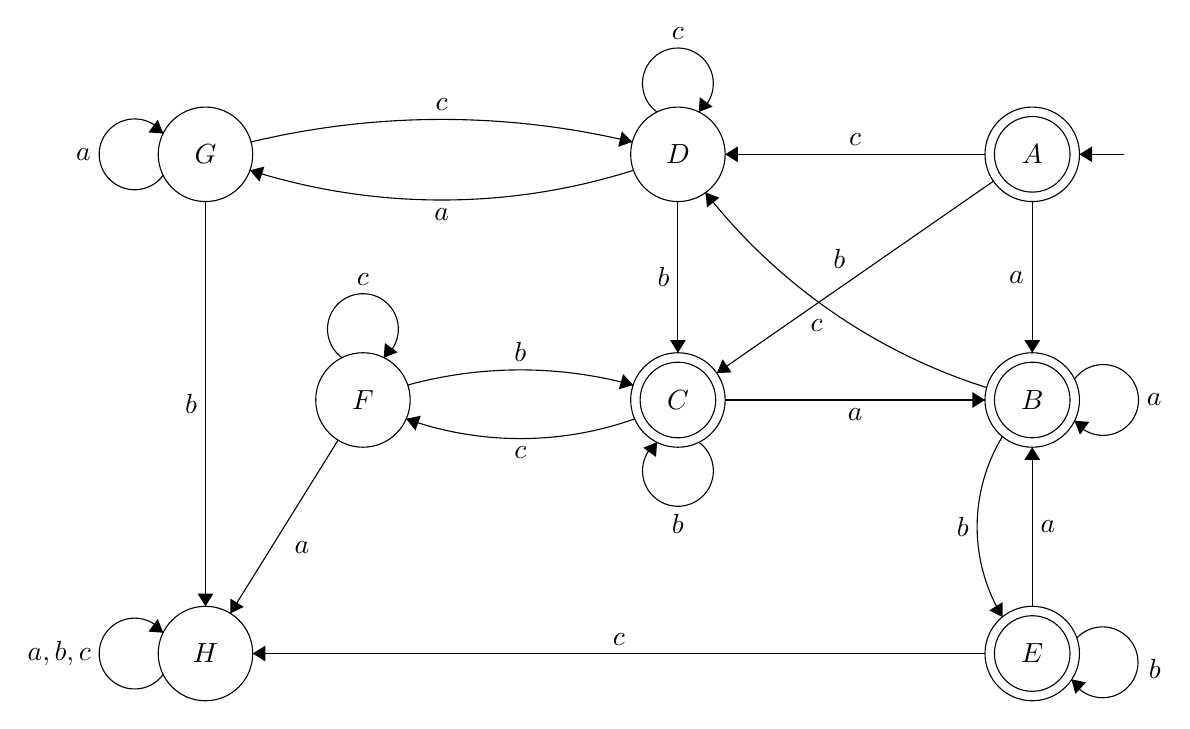
\begin{tikzpicture}[scale=0.2]
\tikzstyle{every node}+=[inner sep=0pt]
\draw [black] (65,-14.8) circle (3);
\draw (65,-14.8) node {$A$};
\draw [black] (65,-14.8) circle (2.4);
\draw [black] (65,-30.4) circle (3);
\draw (65,-30.4) node {$B$};
\draw [black] (65,-30.4) circle (2.4);
\draw [black] (42.5,-30.4) circle (3);
\draw (42.5,-30.4) node {$C$};
\draw [black] (42.5,-30.4) circle (2.4);
\draw [black] (42.5,-14.8) circle (3);
\draw (42.5,-14.8) node {$D$};
\draw [black] (65,-46.5) circle (3);
\draw (65,-46.5) node {$E$};
\draw [black] (65,-46.5) circle (2.4);
\draw [black] (22.5,-30.4) circle (3);
\draw (22.5,-30.4) node {$F$};
\draw [black] (12.5,-14.8) circle (3);
\draw (12.5,-14.8) node {$G$};
\draw [black] (12.5,-46.5) circle (3);
\draw (12.5,-46.5) node {$H$};
\draw [black] (65,-17.8) -- (65,-27.4);
\fill [black] (65,-27.4) -- (65.5,-26.6) -- (64.5,-26.6);
\draw (64.5,-22.6) node [left] {$a$};
\draw [black] (62.53,-16.51) -- (44.97,-28.69);
\fill [black] (44.97,-28.69) -- (45.91,-28.65) -- (45.34,-27.82);
\draw (52.75,-22.1) node [above] {$b$};
\draw [black] (62,-14.8) -- (45.5,-14.8);
\fill [black] (45.5,-14.8) -- (46.3,-15.3) -- (46.3,-14.3);
\draw (53.75,-14.3) node [above] {$c$};
\draw [black] (67.68,-29.077) arc (144:-144:2.25);
\draw (72.25,-30.4) node [right] {$a$};
\fill [black] (67.68,-31.72) -- (68.03,-32.6) -- (68.62,-31.79);
\draw [black] (63.11,-44.182) arc (-148.60922:-211.39078:11.005);
\fill [black] (63.11,-44.18) -- (63.12,-43.24) -- (62.27,-43.76);
\draw (61,-38.45) node [left] {$b$};
\draw [black] (62.106,-29.612) arc (-107.57454:-141.89518:36.815);
\fill [black] (44.25,-17.23) -- (44.35,-18.17) -- (45.14,-17.55);
\draw (51.3,-25.27) node [below] {$c$};
\draw [black] (45.5,-30.4) -- (62,-30.4);
\fill [black] (62,-30.4) -- (61.2,-29.9) -- (61.2,-30.9);
\draw (53.75,-30.9) node [below] {$a$};
\draw [black] (43.823,-33.08) arc (54:-234:2.25);
\draw (42.5,-37.65) node [below] {$b$};
\fill [black] (41.18,-33.08) -- (40.3,-33.43) -- (41.11,-34.02);
\draw [black] (39.753,-31.599) arc (-70.40042:-109.59958:21.621);
\fill [black] (25.25,-31.6) -- (25.83,-32.34) -- (26.17,-31.4);
\draw (32.5,-33.35) node [below] {$c$};
\draw [black] (39.677,-15.814) arc (-72.37536:-107.62464:40.218);
\fill [black] (15.32,-15.81) -- (15.93,-16.53) -- (16.24,-15.58);
\draw (27.5,-18.2) node [below] {$a$};
\draw [black] (42.5,-17.8) -- (42.5,-27.4);
\fill [black] (42.5,-27.4) -- (43,-26.6) -- (42,-26.6);
\draw (42,-22.6) node [left] {$b$};
\draw [black] (41.177,-12.12) arc (234:-54:2.25);
\draw (42.5,-7.55) node [above] {$c$};
\fill [black] (43.82,-12.12) -- (44.7,-11.77) -- (43.89,-11.18);
\draw [black] (65,-43.5) -- (65,-33.4);
\fill [black] (65,-33.4) -- (64.5,-34.2) -- (65.5,-34.2);
\draw (65.5,-38.45) node [right] {$a$};
\draw [black] (67.823,-45.52) arc (136.87498:-151.12502:2.25);
\draw (72.37,-47.47) node [right] {$b$};
\fill [black] (67.49,-48.14) -- (67.74,-49.06) -- (68.42,-48.33);
\draw [black] (62,-46.5) -- (15.5,-46.5);
\fill [black] (15.5,-46.5) -- (16.3,-47) -- (16.3,-46);
\draw (38.75,-46) node [above] {$c$};
\draw [black] (20.92,-32.95) -- (14.08,-43.95);
\fill [black] (14.08,-43.95) -- (14.93,-43.54) -- (14.08,-43.01);
\draw (18.13,-39.74) node [right] {$a$};
\draw [black] (25.344,-29.45) arc (105.29364:74.70636:27.129);
\fill [black] (39.66,-29.45) -- (39.02,-28.76) -- (38.75,-29.72);
\draw (32.5,-27.99) node [above] {$b$};
\draw [black] (21.177,-27.72) arc (234:-54:2.25);
\draw (22.5,-23.15) node [above] {$c$};
\fill [black] (23.82,-27.72) -- (24.7,-27.37) -- (23.89,-26.78);
\draw [black] (9.82,-16.123) arc (-36:-324:2.25);
\draw (5.25,-14.8) node [left] {$a$};
\fill [black] (9.82,-13.48) -- (9.47,-12.6) -- (8.88,-13.41);
\draw [black] (12.5,-17.8) -- (12.5,-43.5);
\fill [black] (12.5,-43.5) -- (13,-42.7) -- (12,-42.7);
\draw (12,-30.65) node [left] {$b$};
\draw [black] (15.395,-14.016) arc (103.50114:76.49886:51.848);
\fill [black] (39.6,-14.02) -- (38.94,-13.34) -- (38.71,-14.32);
\draw (27.5,-12.08) node [above] {$c$};
\draw [black] (9.82,-47.823) arc (324:36:2.25);
\draw (5.25,-46.5) node [left] {$a,b,c$};
\fill [black] (9.82,-45.18) -- (9.47,-44.3) -- (8.88,-45.11);
\draw [black] (70.8,-14.8) -- (68,-14.8);
\fill [black] (68,-14.8) -- (68.8,-15.3) -- (68.8,-14.3);
\end{tikzpicture}
\newline
\end{center}

\subsection*{(ب)}
همانطور که در صورت سوال ذکر شده است نیازی نیست تمامی حالات را بررسی کنیم. بنابراین از 
\lr{$\epsilon$-closure} استیت آغازین شروع به حرکت کرده و در هر مرحله که استیت جدیدی اضافه شد، مراحل مشابه را برای آن تکرار می‌نماییم تا جایی که استیت جدید دیگری تولید نشود.
داریم: \newline

\begin{center}
    \begin{equation*}
    \begin{cases}
        \delta &=
        \begin{tabular}{c|c|c}
         & $a$ & $b$\\ \hline
        $\{0,1,2\}$ & $\{1,2,3,4\}$ &$\{1,2\}$\\
        $\{1,2,3,4\}$ & $\{1,2,3,4,6\}$ &$\{1,2,5\}$\\
        $\{1,2\}$ & $\{1,2,3,4\}$ &$\{1,2\}$\\
        $\{1,2,3,4,6\}$ & $\{1,2,3,4,6,7\}$ &$\{1,2,5\}$\\
        $\{1,2,5\}^*$ & $\{1,2,3,4\}$ &$\{1,2\}$\\
        $\{1,2,3,4,6,7\}^*$ & $\{1,2,3,4,6,7\}$ &$\{1,2,5,7\}$\\
        $\{1,2,5,7\}^*$ & $\{1,2,3,4,7\}$ &$\{1,2,7\}$\\
        $\{1,2,3,4,7\}^*$ & $\{1,2,3,4,6,7\}$ &$\{1,2,5,7\}$\\
        $\{1,2,7\}^*$ & $\{1,2,3,4,7\}$ &$\{1,2,7\}$\\
        \end{tabular}\\[0.2in]
        Q &= \{ A=\{0,1,2\},\; B=\{1,2,3,4\},\;C=\{1,2\},\\
        &\;\;\;\; D=\{1,2,3,4,6\},\;
        E=\{1,2,5\},\; F=\{1,2,3,4,6,7\},\\
        &\;\;\;\; \;G=\{1,2,5,7\},\;H=\{1,2,3,4,7\},\; I=\{1,2,7\}\}\\
        \Sigma &= \{ a, b\} \\
        q_0 &= A\\
        F &= \{E,\;F,\;G,\;H,\; I\}\\
    \end{cases}
    \end{equation*}
    $M = (Q, \Sigma, \delta, q_0, F)$
    \\[0.3in]
\end{center}
حال $DFA$ را رسم می‌کنیم. دقت کنید در جدول بالا، علامت * به معنای نهایی بودن آن استیت می‌باشد.

\begin{center}
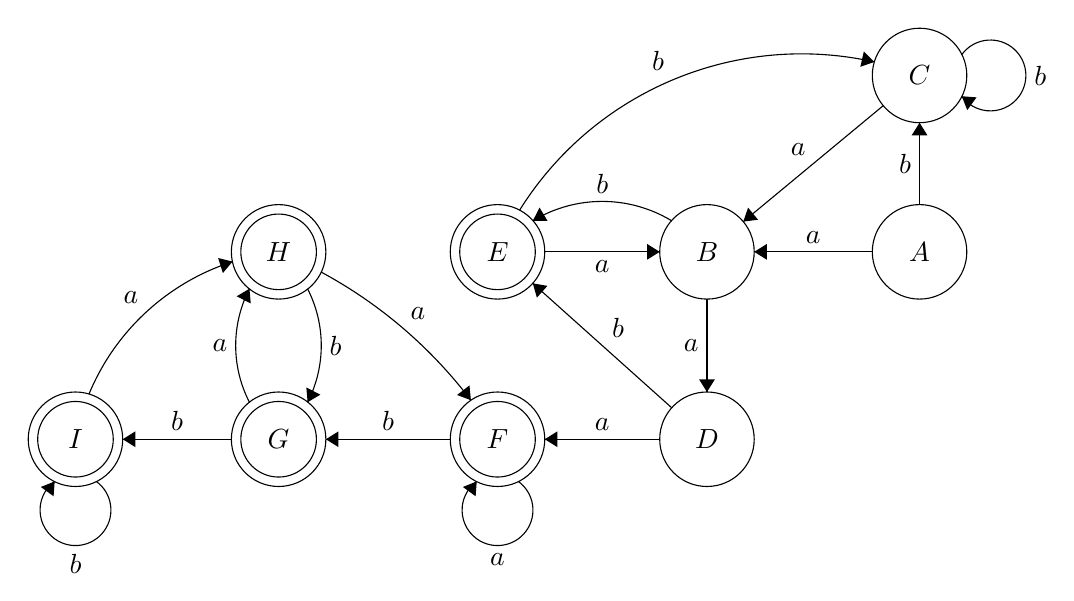
\begin{tikzpicture}[scale=0.2]
\tikzstyle{every node}+=[inner sep=0pt]
\draw [black] (64.8,-15.1) circle (3);
\draw (64.8,-15.1) node {$A$};
\draw [black] (51.3,-15.1) circle (3);
\draw (51.3,-15.1) node {$B$};
\draw [black] (64.8,-3.9) circle (3);
\draw (64.8,-3.9) node {$C$};
\draw [black] (51.3,-27) circle (3);
\draw (51.3,-27) node {$D$};
\draw [black] (38,-15.1) circle (3);
\draw (38,-15.1) node {$E$};
\draw [black] (38,-15.1) circle (2.4);
\draw [black] (38,-27) circle (3);
\draw (38,-27) node {$F$};
\draw [black] (38,-27) circle (2.4);
\draw [black] (24.1,-27) circle (3);
\draw (24.1,-27) node {$G$};
\draw [black] (24.1,-27) circle (2.4);
\draw [black] (24.1,-15.1) circle (3);
\draw (24.1,-15.1) node {$H$};
\draw [black] (24.1,-15.1) circle (2.4);
\draw [black] (11.2,-27) circle (3);
\draw (11.2,-27) node {$I$};
\draw [black] (11.2,-27) circle (2.4);
\draw [black] (61.8,-15.1) -- (54.3,-15.1);
\fill [black] (54.3,-15.1) -- (55.1,-15.6) -- (55.1,-14.6);
\draw (58.05,-14.6) node [above] {$a$};
\draw [black] (64.8,-12.1) -- (64.8,-6.9);
\fill [black] (64.8,-6.9) -- (64.3,-7.7) -- (65.3,-7.7);
\draw (64.3,-9.5) node [left] {$b$};
\draw [black] (51.3,-18.1) -- (51.3,-24);
\fill [black] (51.3,-24) -- (51.8,-23.2) -- (50.8,-23.2);
\draw (50.8,-21.05) node [left] {$a$};
\draw [black] (40.241,-13.129) arc (121.23212:58.76788:8.504);
\fill [black] (40.24,-13.13) -- (41.18,-13.14) -- (40.67,-12.29);
\draw (44.65,-11.4) node [above] {$b$};
\draw [black] (62.49,-5.82) -- (53.61,-13.18);
\fill [black] (53.61,-13.18) -- (54.54,-13.06) -- (53.91,-12.29);
\draw (57.1,-9.01) node [above] {$a$};
\draw [black] (67.48,-2.577) arc (144:-144:2.25);
\draw (72.05,-3.9) node [right] {$b$};
\fill [black] (67.48,-5.22) -- (67.83,-6.1) -- (68.42,-5.29);
\draw [black] (48.3,-27) -- (41,-27);
\fill [black] (41,-27) -- (41.8,-27.5) -- (41.8,-26.5);
\draw (44.65,-26.5) node [above] {$a$};
\draw [black] (49.06,-25) -- (40.24,-17.1);
\fill [black] (40.24,-17.1) -- (40.5,-18.01) -- (41.17,-17.26);
\draw (45.66,-20.56) node [above] {$b$};
\draw [black] (41,-15.1) -- (48.3,-15.1);
\fill [black] (48.3,-15.1) -- (47.5,-14.6) -- (47.5,-15.6);
\draw (44.65,-15.6) node [below] {$a$};
\draw [black] (39.404,-12.452) arc (147.99141:77.36971:21.118);
\fill [black] (61.93,-3.04) -- (61.26,-2.38) -- (61.04,-3.35);
\draw (48.2,-3.65) node [above] {$b$};
\draw [black] (39.323,-29.68) arc (54:-234:2.25);
\draw (38,-34.25) node [below] {$a$};
\fill [black] (36.68,-29.68) -- (35.8,-30.03) -- (36.61,-30.62);
\draw [black] (35,-27) -- (27.1,-27);
\fill [black] (27.1,-27) -- (27.9,-27.5) -- (27.9,-26.5);
\draw (31.05,-26.5) node [above] {$b$};
\draw [black] (22.252,-24.66) arc (-152.63846:-207.36154:7.855);
\fill [black] (22.25,-17.44) -- (21.44,-17.92) -- (22.33,-18.38);
\draw (20.87,-21.05) node [left] {$a$};
\draw [black] (21.1,-27) -- (14.2,-27);
\fill [black] (14.2,-27) -- (15,-27.5) -- (15,-26.5);
\draw (17.65,-26.5) node [above] {$b$};
\draw [black] (26.808,-16.388) arc (61.65663:37.2087:29.539);
\fill [black] (36.31,-24.52) -- (36.22,-23.58) -- (35.43,-24.19);
\draw (32.95,-19.46) node [above] {$a$};
\draw [black] (25.938,-17.448) arc (27.15687:-27.15687:7.891);
\fill [black] (25.94,-24.65) -- (26.75,-24.17) -- (25.86,-23.71);
\draw (27.31,-21.05) node [right] {$b$};
\draw [black] (12.059,-24.131) arc (157.51945:107.86242:14.762);
\fill [black] (21.17,-15.72) -- (20.26,-15.49) -- (20.56,-16.45);
\draw (14.73,-18.44) node [above] {$a$};
\draw [black] (12.523,-29.68) arc (54:-234:2.25);
\draw (11.2,-34.25) node [below] {$b$};
\fill [black] (9.88,-29.68) -- (9,-30.03) -- (9.81,-30.62);
\end{tikzpicture}
\newline
\end{center}

در حل سوال به 2 نکته زیر توجه شده است:
\begin{itemize}
    \item استیت‌های قابل دسترس، گام به گام و به ترتیب اضافه شده‌اند.
    \item DFA های به‌ دست آمده حالات کوتاه شده‌تر نیز دارند که به دلیل اینکه خواسته سوال نبوده است، صرفا به حالت کلی بسنده کرده‌ایم.
\end{itemize}

* نکته: در $DFA$ دوم، فراموش شده است که استیت $A$ به عنوان حالت شروع ذکر بشود، اما در تعریف آن به $q_0\;=\;A$ اشاره کرده‌ایم و همین متن نیز مجدد به آن اشاره دارد :).\\